% !TEX root = ../proyect.tex

\chapter{Manuales}\label{cap:manuales}

Un sistema de software no se considera completo si quienes han de utilizarlo, mantenerlo o evolucionarlo no disponen de instrucciones suficientes para hacerlo. Por ese motivo, este capítulo recoge tres manuales complementarios que cubren los tres perfiles de interacción previstos para Linceus Assistant. El \textbf{manual de usuario} se dirige al alumnado de la ETSII, principal destinatario del prototipo, y describe cómo formular consultas y aprovechar las funcionalidades disponibles. El \textbf{manual de despliegue} se dirige al personal técnico encargado de instalar y mantener el sistema, y detalla los requisitos, procedimientos y comprobaciones necesarias para poner en marcha la plataforma. El \textbf{manual de desarrollo}, por último, se dirige a los futuros estudiantes, becarios o investigadores que continúen este trabajo, y describe la organización del repositorio, las convenciones de codificación y el ciclo de incorporación de nuevos cambios.

Los tres manuales se basan en el estado del proyecto a fecha del cierre del prototipo (26 de abril de 2026). Cualquier divergencia con el repositorio actual debe consultarse en los ficheros \texttt{README.md} y \texttt{docker-compose.yml}, que son las referencias técnicas autoritativas y se mantienen actualizadas con los cambios del proyecto.

% =====================================================
% SECCIÓN 1: MANUAL DE USUARIO
% =====================================================
\section{Manual de usuario}\label{sec:manual-usuario}

El destinatario de este manual es el alumnado de la ETSII que utiliza Linceus Assistant para resolver dudas académicas. El manual describe la interfaz, el modelo conversacional y los flujos de consulta disponibles, sin entrar en detalles técnicos de implementación.

\subsection{Acceso a la aplicación}\label{subsec:usuario-acceso}

Linceus Assistant se ofrece como una aplicación web responsiva, accesible desde cualquier navegador moderno (Chrome, Firefox, Edge, Safari) tanto en ordenador como en dispositivo móvil. La página principal del prototipo muestra una breve descripción del proyecto y un \textit{widget} de chat anclado en la esquina inferior derecha, que se despliega al hacer clic sobre el icono (Figura~\ref{fig:widget-cerrado}). No se requiere autenticación previa: la sesión se identifica internamente mediante un identificador anónimo generado por el navegador, lo que permite mantener el contexto durante la conversación sin recoger datos personales.

\begin{figure}[hbtp]
  \centering
  % CAPTURA: pantalla completa del prototipo con el widget cerrado (botón azul
  % redondo en esquina inferior derecha visible). Navegador sin barra de URL.
  % Guardar como: img/widget_cerrado.png
  
\includegraphics[width=0.95\linewidth]{img/widget_cerrado.png}
  \caption{Página principal del prototipo con el \textit{widget} de chat cerrado.}
  \label{fig:widget-cerrado}
\end{figure}

Tras desplegar el chat, el alumno encuentra un mensaje de bienvenida y, sobre él, un selector de titulación que sirve para fijar el contexto académico inicial (Figura~\ref{fig:widget-abierto}). Por defecto, la titulación seleccionada es Grado en Ingeniería Informática -- Ingeniería del Software (GII-IS), por ser la titulación con mayor cobertura informativa en el prototipo, pero el alumno puede cambiarla en cualquier momento, ya sea desde el selector o expresando el cambio en lenguaje natural durante la conversación (``cambia a tecnologías informáticas'', ``soy de IC'').

\begin{figure}[hbtp]
  \centering
  % CAPTURA: widget abierto, con el mensaje de bienvenida y el selector de
  % titulación visible. Sin conversación iniciada aún.
  % Guardar como: img/widget_abierto.png
  
\includegraphics[width=0.95\linewidth]{img/widget_abierto.png}
  \caption{\textit{Widget} desplegado con mensaje de bienvenida y selector de titulación.}
  \label{fig:widget-abierto}
\end{figure}

\subsection{Modelo conversacional}\label{subsec:usuario-modelo}

El asistente está diseñado para responder a consultas formuladas en español natural. No es necesario emplear comandos ni una sintaxis específica: el sistema interpreta la intención del usuario a partir del texto libre y se apoya en el contexto de los turnos anteriores cuando la consulta es elíptica. Esto significa, por ejemplo, que tras preguntar por una asignatura concreta el alumno puede continuar con preguntas como ``¿y cuántos créditos tiene?'' sin necesidad de repetir el nombre.

El bot tolera errores tipográficos moderados, abreviaturas habituales (FP, ADDA, IISSI2, PSG2) y reformulaciones de la misma pregunta. Ante una consulta ambigua, el asistente solicita al usuario los datos que necesita, típicamente el curso o el grupo cuando la consulta afecta a horarios. Si la información solicitada no está disponible en la base de datos, el bot responde de forma explícita, sin inventar contenido. Las preguntas que caen fuera del ámbito académico (información meteorológica, peticiones generales no relacionadas con la universidad) se rechazan con un mensaje cortés y se redirige al usuario hacia el conjunto de funcionalidades soportadas.

\subsection{Funcionalidades disponibles}\label{subsec:usuario-funcionalidades}

El prototipo cubre tres dominios funcionales principales. La Tabla~\ref{tab:funcionalidades-usuario} resume los tipos de consulta soportados con un ejemplo representativo de cada uno.

\begin{table}[hbtp]
\centering
\caption{Tipos de consulta soportados por el prototipo.}\label{tab:funcionalidades-usuario}
\begin{tabular}{p{3.4cm}p{4cm}p{6cm}}
\hline
\textbf{Dominio} & \textbf{Tipo de consulta} & \textbf{Ejemplo de pregunta} \\
\hline
Asignaturas & Ficha individual & ``¿Qué es ADDA?'' \\
 & Listado por criterio & ``¿Qué optativas hay en cuarto?'' \\
 & Conteo & ``¿Cuántas obligatorias tiene tercero?'' \\
 & Información del plan docente & ``¿Cómo se evalúa PSG2?'' \\
\hline
Horarios & Por curso y grupo & ``Horario de segundo grupo 3'' \\
 & Por asignatura & ``¿Cuándo es ADDA?'' \\
 & Por día concreto & ``¿Qué clases hay el lunes?'' \\
 & Por aula o laboratorio & ``Laboratorio de Álgebra grupo 1'' \\
\hline
Profesorado & Datos de contacto & ``Email de Galindo'' \\
 & Profesores de una asignatura & ``¿Quiénes imparten IISSI2?'' \\
 & Coordinación & ``¿Quién coordina IA?'' \\
 & Tutorías & ``Tutorías de Bernárdez'' \\
\hline
\end{tabular}
\end{table}

Más allá de estas funcionalidades primarias, el bot incorpora dos comportamientos transversales que conviene conocer. El primero es el \textit{cambio de contexto académico}, ya mencionado, que permite consultar información de cualquiera de las tres titulaciones de la ETSII (Ingeniería del Software, Ingeniería de Computadores, Tecnologías Informáticas) cambiando dinámicamente la titulación activa. El segundo es el \textit{seguimiento conversacional}, que permite formular consultas elípticas apoyadas en los turnos anteriores: tras preguntar por una asignatura, expresiones del tipo ``¿y de qué curso es?'', ``¿y los profesores?'' o ``¿y el horario?'' resuelven correctamente la referencia implícita. La Figura~\ref{fig:conversacion-ejemplo} muestra una sesión representativa con varias de estas capacidades encadenadas.

\begin{figure}[hbtp]
  \centering
  % CAPTURA: conversación real en el widget que muestre al menos:
  %   - una consulta de asignatura (p.ej. "¿qué es ADDA?")
  %   - una pregunta de seguimiento elíptica (p.ej. "¿y cuántos créditos?")
  %   - una consulta de profesorado o cambio de titulación
  % Guardar como: img/conversacion_ejemplo.png
  
\includegraphics[width=0.95\linewidth]{img/conversacion_ejemplo.png}
  \caption{Ejemplo de sesión con seguimiento conversacional y cambio de contexto.}
  \label{fig:conversacion-ejemplo}
\end{figure}

\subsection{Recomendaciones de uso}\label{subsec:usuario-recomendaciones}

Aunque el sistema admite formulaciones libres, la calidad de la respuesta mejora cuando el alumno aporta el contexto necesario en la propia consulta. Para horarios resulta útil indicar curso y grupo desde el primer turno; para profesorado, el apellido completo o el nombre exacto reduce la ambigüedad cuando varios docentes comparten apellido. Las consultas demasiado abiertas (``cuéntame cosas de la carrera'') tienden a producir respuestas genéricas, ya que el bot no dispone de un único objetivo informativo al que dirigirse. Por último, el sistema no almacena el contenido de las conversaciones para fines comerciales y permite al usuario reportar respuestas incorrectas mediante el botón de \textit{feedback} integrado en cada turno, lo cual contribuye a la mejora continua del prototipo.

\subsection{Panel de administración}\label{subsec:usuario-admin}

El sistema incluye un panel de administración accesible en \texttt{/admin.html}, protegido por autenticación, que permite gestionar los datos académicos del prototipo sin necesidad de acceder directamente a la base de datos. El panel se organiza en cinco secciones accesibles desde la barra de navegación superior.

La vista de inicio (Figura~\ref{fig:admin-home}) muestra la jerarquía de centros y titulaciones disponibles. Desde ella se puede navegar a las asignaturas de cada titulación y consultar o actualizar su información.

\begin{figure}[hbtp]
  \centering
  
\includegraphics[width=0.95\linewidth]{img/admin_home.png}
  \caption{Panel de administración: vista de centros y titulaciones.}
  \label{fig:admin-home}
\end{figure}

La sección de profesores (Figura~\ref{fig:admin-profesores}) lista el profesorado con sus datos de contacto y permite actualizar la información directamente desde el panel, sin necesidad de re-entrenar el modelo.

\begin{figure}[hbtp]
  \centering
  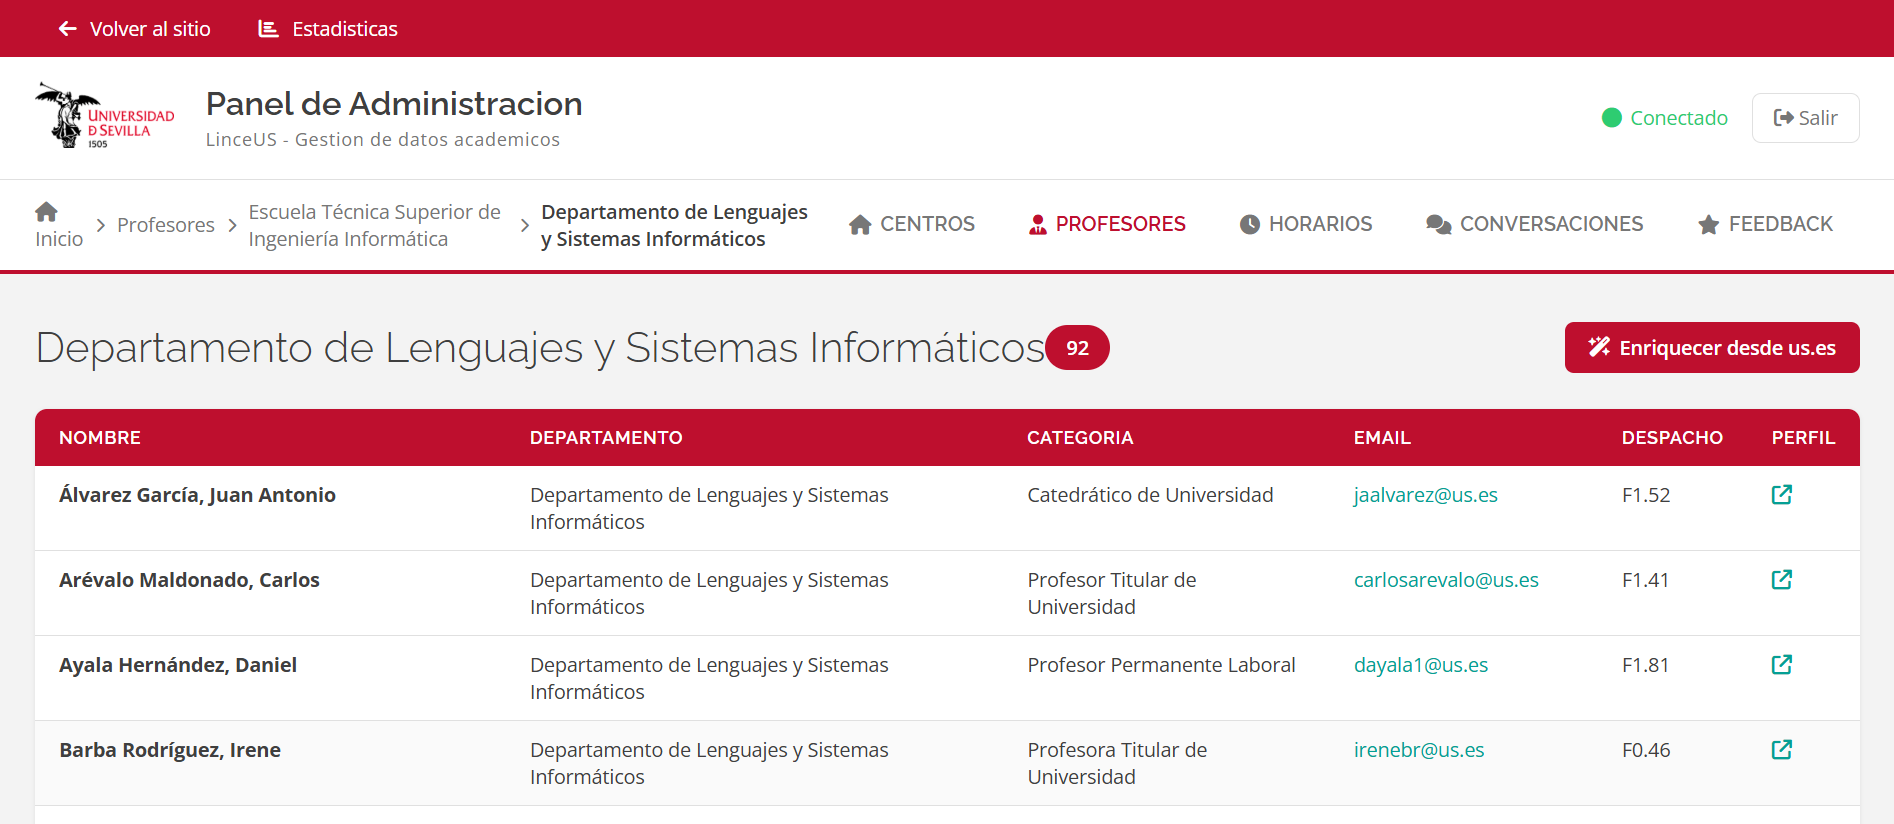
\includegraphics[width=0.95\linewidth]{img/admin_profesores.png}
  \caption{Panel de administración: gestión del profesorado.}
  \label{fig:admin-profesores}
\end{figure}

La sección de horarios (Figura~\ref{fig:man-admin-horarios}) muestra los horarios estructurados por titulación, curso y grupo, y expone los mismos datos que el chatbot consulta en tiempo real.

\begin{figure}[hbtp]
  \centering
  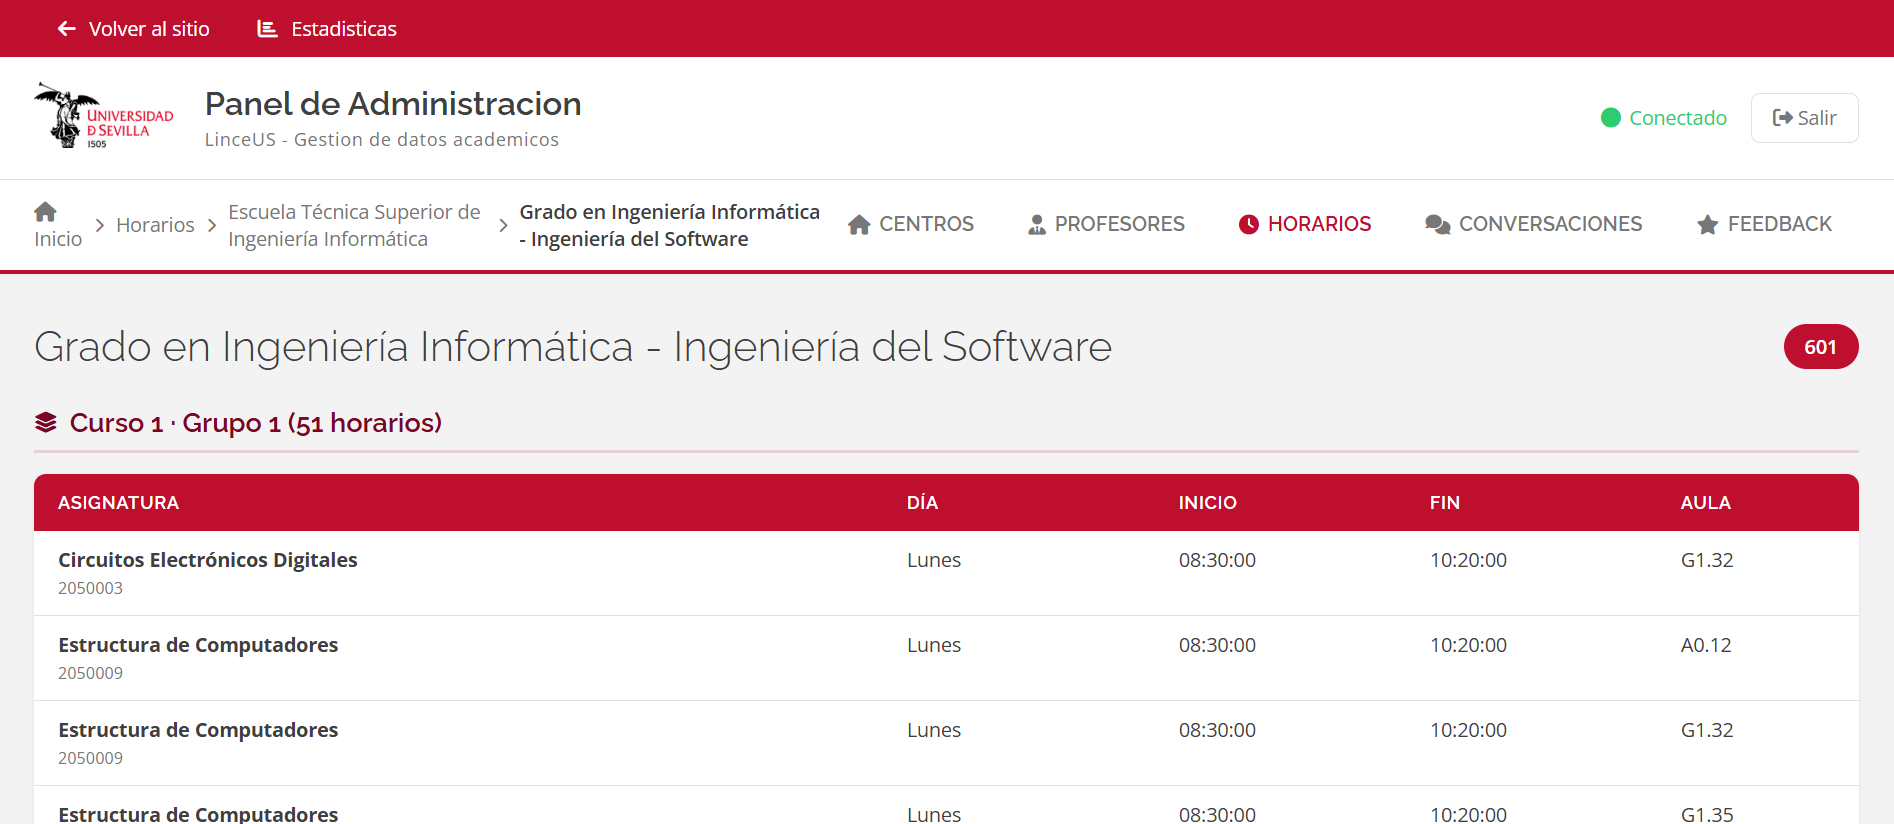
\includegraphics[width=0.95\linewidth]{img/admin_horarios.png}
  \caption{Panel de administración: vista de horarios.}
  \label{fig:man-admin-horarios}
\end{figure}

La sección de conversaciones (Figura~\ref{fig:man-admin-conversaciones}) registra las sesiones de usuario de forma anonimizada, lo que permite detectar patrones de uso, preguntas frecuentes y casos en los que el bot no proporcionó una respuesta satisfactoria.

\begin{figure}[hbtp]
  \centering
  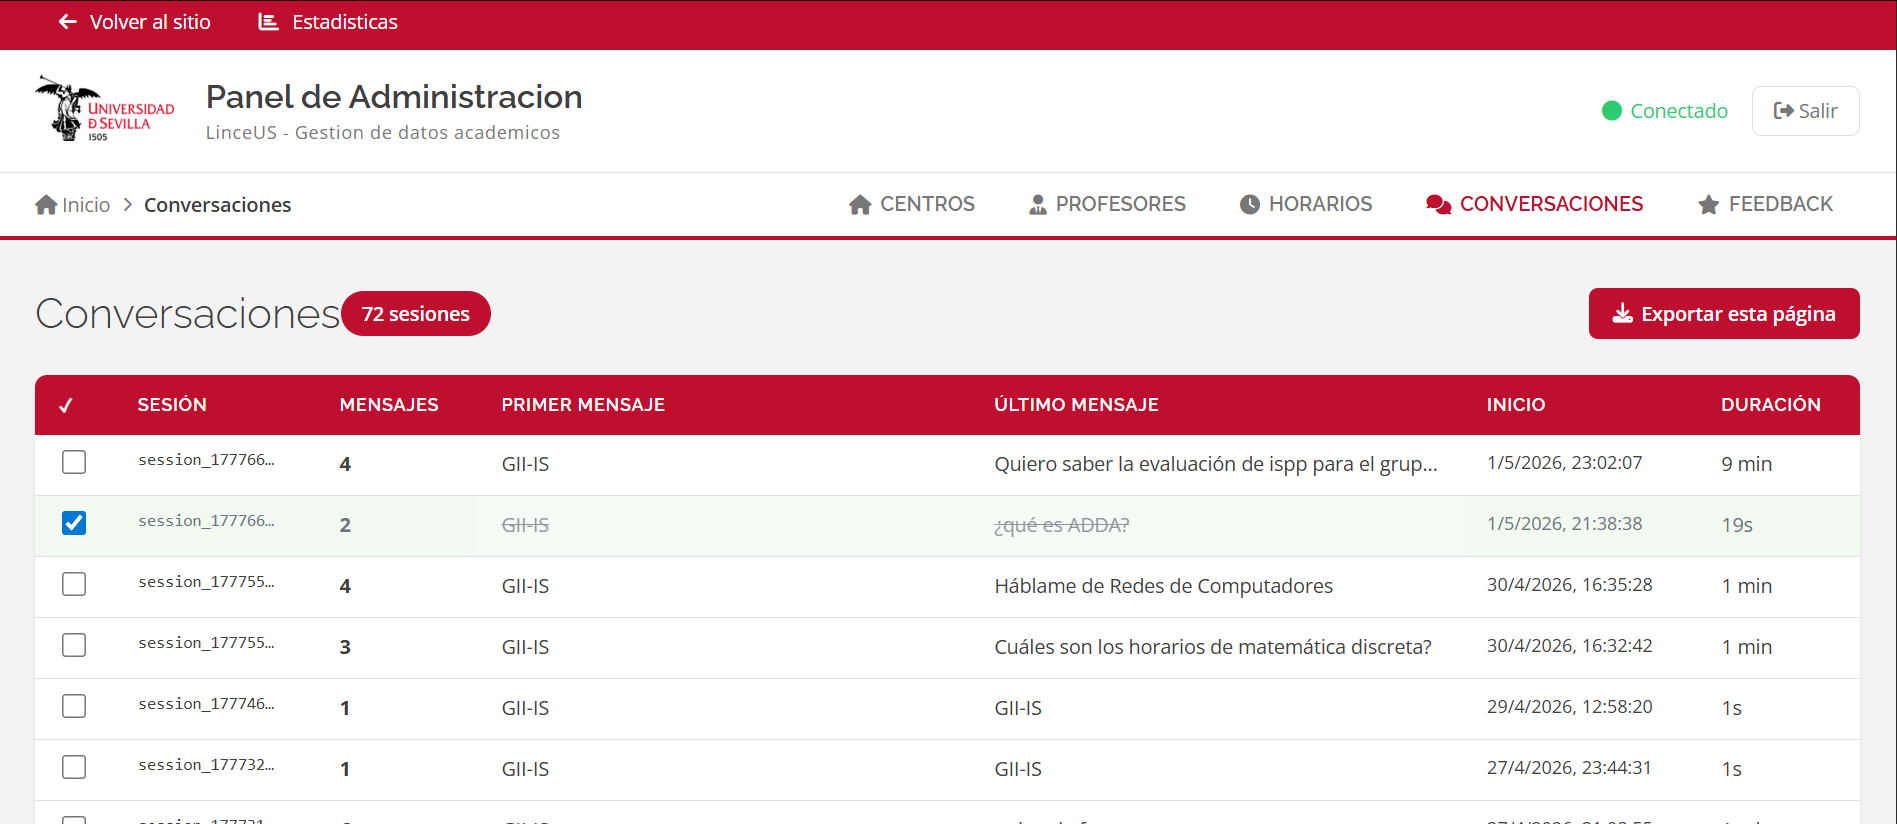
\includegraphics[width=0.95\linewidth]{img/admin_conversaciones.png}
  \caption{Panel de administración: registro de conversaciones anonimizadas.}
  \label{fig:man-admin-conversaciones}
\end{figure}

Por último, la vista de estadísticas (Figura~\ref{fig:admin-stats}) agrega métricas de uso del sistema: número de sesiones, distribución de intenciones detectadas y evolución temporal del tráfico.

\begin{figure}[hbtp]
  \centering
  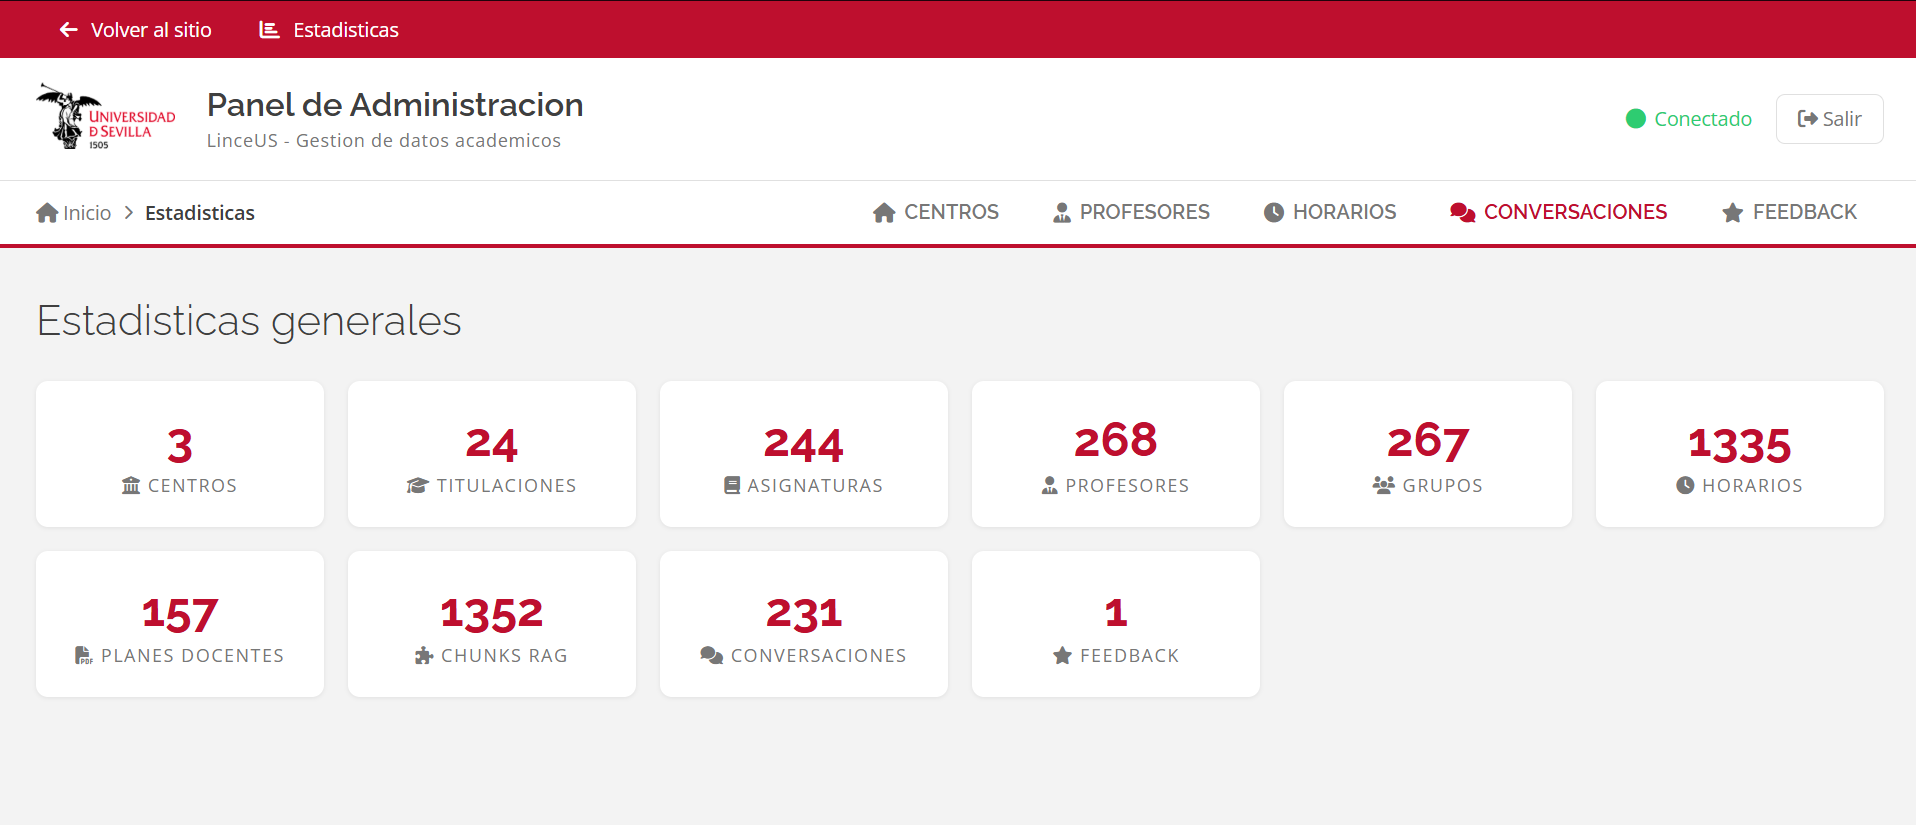
\includegraphics[width=0.95\linewidth]{img/admin_stats.png}
  \caption{Panel de administración: estadísticas de uso del sistema.}
  \label{fig:admin-stats}
\end{figure}

% =====================================================
% SECCIÓN 2: MANUAL DE DESPLIEGUE
% =====================================================
\section{Manual de despliegue}\label{sec:manual-despliegue}

El manual de despliegue describe los pasos necesarios para instalar Linceus Assistant en una infraestructura nueva, ya sea un entorno de desarrollo local o un servidor de producción. La instalación se ha diseñado para ser reproducible mediante Docker Compose, lo que evita la necesidad de instalar manualmente el conjunto de dependencias del \textit{stack} y reduce drásticamente las divergencias entre entornos.

\subsection{Requisitos previos}\label{subsec:despliegue-requisitos}

La máquina destinataria debe cumplir los requisitos mínimos recogidos en la Tabla~\ref{tab:despliegue-requisitos}. Estos requisitos se han validado sobre el \textit{droplet} de DigitalOcean utilizado durante el piloto y son suficientes para la carga prevista en la fase de prototipo (un orden de magnitud por debajo de la población total de la ETSII).

\begin{table}[hbtp]
\centering
\caption{Requisitos mínimos del entorno de despliegue.}\label{tab:despliegue-requisitos}
\begin{tabular}{ll}
\hline
\textbf{Recurso} & \textbf{Valor recomendado} \\
\hline
Sistema operativo & Linux (Ubuntu 22.04 LTS o equivalente) \\
CPU & 2 vCPU \\
Memoria RAM & 4 GB \\
Almacenamiento & 20 GB SSD \\
Docker Engine & 24.x o superior \\
Docker Compose & v2 (incluido en Docker Engine) \\
Conectividad saliente & HTTPS hacia Supabase y Google AI Studio \\
\hline
\end{tabular}
\end{table}

Además de los recursos de cómputo, el despliegue requiere disponer de tres credenciales externas: la cadena de conexión a la base de datos Supabase con extensión \texttt{pgvector}, la clave de API de Google AI Studio para el modelo Gemini y un dominio o subdominio con certificado TLS si la instalación se realiza en producción. Estas credenciales se configuran en un fichero \texttt{.env} ubicado en la raíz del proyecto, cuyo formato se describe en \texttt{.env.example}.

\subsection{Instalación}\label{subsec:despliegue-instalacion}

La instalación parte de la clonación del repositorio del proyecto y se completa en cuatro pasos. El primer paso consiste en obtener una copia local del código y situarse en el directorio resultante. El segundo paso es preparar el fichero \texttt{.env} a partir de la plantilla, sustituyendo cada variable por el valor correspondiente al entorno de despliegue. El tercer paso es asegurarse de que el directorio \texttt{models/} contiene un modelo Rasa entrenado: si no es así, basta con ejecutar \texttt{rasa train} en un entorno con las dependencias instaladas, o bien copiar el último modelo válido desde el repositorio. El cuarto y último paso es levantar la pila completa con Docker Compose:

\begin{lstlisting}[language=bash, caption={Levantar la pila completa con Docker Compose.}]
git clone <url-repositorio> && cd linceus-assistant
cp .env.example .env          # completar variables
docker compose -f docker/docker-compose.yml up --build -d
\end{lstlisting}

La opción \texttt{-d} ejecuta los contenedores en segundo plano. El primer arranque construye las imágenes correspondientes, lo que puede tardar varios minutos en función del ancho de banda disponible para descargar las dependencias. A partir de ese momento, los rearranques posteriores son cuestión de pocos segundos, salvo que se hayan modificado las dependencias de Python.

\subsection{Arquitectura del despliegue}\label{subsec:despliegue-arquitectura}

La pila se compone de cuatro contenedores que se comunican entre sí a través de la red interna de Docker, recogidos en la Tabla~\ref{tab:despliegue-contenedores}. Únicamente el contenedor de \textit{frontend} expone el puerto 80 al exterior; el resto de servicios son accesibles solo desde el interior de la red, salvo que el operador decida exponerlos explícitamente para fines de depuración.

\begin{table}[hbtp]
\centering
\caption{Contenedores del despliegue y responsabilidad de cada uno.}\label{tab:despliegue-contenedores}
\begin{tabular}{llll}
\hline
\textbf{Contenedor} & \textbf{Imagen base} & \textbf{Versión} & \textbf{Responsabilidad} \\
\hline
\texttt{frontend} & \texttt{nginx:alpine} & alpine & Sirve los ficheros estáticos y actúa como \textit{proxy} \\
\texttt{rasa} & \texttt{rasa/rasa} & 3.6.21 + spaCy & Gestor del diálogo y NLU (puerto 5005) \\
\texttt{actions} & \texttt{python:3.10.14-slim-bookworm} & 3.10.14 & Acciones personalizadas y módulo RAG \\
\texttt{admin} & \texttt{python:3.10-slim} & 3.10 & API Flask del panel de administración \\
\hline
\end{tabular}
\end{table}

El contenedor de \textit{actions} monta los directorios \texttt{actions/} y \texttt{rag/} como volúmenes, lo que permite recargar los cambios en caliente sin reconstruir la imagen. El contenedor de Rasa monta los ficheros de configuración (\texttt{config.yml}, \texttt{domain.yml}, \texttt{credentials.yml}) y un fichero específico de \textit{endpoints} que enruta el servidor hacia el contenedor de \textit{actions} a través del nombre de servicio interno. El contenedor de \textit{frontend} inyecta la variable \texttt{RASA\_SERVER} en los ficheros estáticos en el momento del arranque mediante un \textit{script} de \textit{entrypoint}, lo que evita tener que recompilar el \textit{frontend} para distintos entornos.

\subsection{Verificación del despliegue}\label{subsec:despliegue-verificacion}

Una vez levantada la pila, la verificación del despliegue se realiza siguiendo cuatro comprobaciones en orden. En primer lugar, la página principal debe estar accesible en \texttt{http://<host>/}, donde \texttt{<host>} es la dirección o dominio del servidor. En segundo lugar, el panel de administración debe estar accesible en \texttt{http://<host>/admin.html} y permitir consultar la lista de centros y titulaciones. En tercer lugar, el \textit{widget} de chat debe responder a un mensaje de prueba simple (``hola'') con un saludo personalizado, lo cual confirma que el camino completo entre \textit{frontend}, Rasa, \textit{actions} y modelo Gemini está operativo. Por último, una consulta sencilla con dependencia de base de datos (``¿cuántas asignaturas tiene primero?'') debe devolver una cifra coherente con los datos cargados, lo cual confirma la conectividad con Supabase.

Si alguna de estas comprobaciones falla, los registros de cada contenedor se consultan con la orden recogida en el Código~\ref{lst:logs}, donde \texttt{<servicio>} es uno de los cuatro nombres recogidos en la Tabla~\ref{tab:despliegue-contenedores}. El error más habitual durante la primera puesta en marcha es la falta de un modelo entrenado en \texttt{models/}, lo que provoca que el contenedor de Rasa se reinicie en bucle.

\begin{lstlisting}[language=bash, caption={Consultar registros de un contenedor.}, label={lst:logs}]
docker compose -f docker/docker-compose.yml logs -f <servicio>
# Ejemplo: ver logs del servidor Rasa en tiempo real
docker compose -f docker/docker-compose.yml logs -f rasa
\end{lstlisting}

\subsection{Operaciones habituales}\label{subsec:despliegue-operaciones}

El día a día del operador se concentra en un puñado de tareas rutinarias. Los cambios en el código de \textit{actions} o del módulo RAG no requieren reiniciar nada, ya que el \textit{action server} se ejecuta con la opción \texttt{--auto-reload}. Los cambios en el modelo Rasa (re-entrenamiento) requieren detener y volver a arrancar el contenedor \texttt{rasa} para que recargue el modelo desde el volumen \texttt{models/}. Las actualizaciones de las dependencias de Python requieren reconstruir la imagen afectada antes de volver a levantarla. Las copias de seguridad de la base de datos se gestionan desde el panel de Supabase, que dispone de \textit{snapshots} automáticos diarios; el código del proyecto no almacena estado mutable en disco fuera de la base de datos.

\begin{lstlisting}[language=bash, caption={Operaciones de mantenimiento habituales.}]
# Recargar modelo Rasa tras reentrenamiento
docker compose -f docker/docker-compose.yml restart rasa

# Reconstruir imagen tras cambio de dependencias Python
docker compose -f docker/docker-compose.yml build actions
docker compose -f docker/docker-compose.yml up -d actions

# Detener toda la pila
docker compose -f docker/docker-compose.yml down
\end{lstlisting}

% =====================================================
% SECCIÓN 3: MANUAL DE DESARROLLO
% =====================================================
\section{Manual de desarrollo}\label{sec:manual-desarrollo}

El manual de desarrollo se dirige a quien deba modificar, ampliar o mantener el código de Linceus Assistant tras el cierre de este TFG. Su objetivo es minimizar la curva de aprendizaje proporcionando una visión panorámica del repositorio, las convenciones empleadas y el ciclo de trabajo recomendado.

\subsection{Estructura del repositorio}\label{subsec:desarrollo-estructura}

El repositorio sigue la disposición habitual de un proyecto Rasa con extensiones específicas para el módulo RAG y el panel de administración. La Tabla~\ref{tab:desarrollo-estructura} recoge los directorios de primer nivel y su responsabilidad.

\begin{table}[hbtp]
\centering
\caption{Estructura del repositorio Linceus Assistant.}\label{tab:desarrollo-estructura}
\begin{tabular}{ll}
\hline
\textbf{Directorio} & \textbf{Contenido} \\
\hline
\texttt{actions/} & Acciones personalizadas (Python) que ejecuta el \textit{action server} \\
\texttt{admin/} & Aplicación Flask del panel de administración \\
\texttt{data/} & Conjuntos de datos NLU y \textit{stories} para Rasa \\
\texttt{docker/} & Ficheros de Compose y \textit{Dockerfile} de cada servicio \\
\texttt{frontend/} & \textit{Widget} de chat y panel HTML/CSS/JS \\
\texttt{models/} & Modelos Rasa entrenados (no versionados) \\
\texttt{rag/} & Módulo de recuperación aumentada por generación \\
\texttt{tests/} & Suite de aceptación funcional y planes de prueba \\
\hline
\end{tabular}
\end{table}

Los ficheros de configuración principales (\texttt{config.yml}, \texttt{domain.yml}, \texttt{credentials.yml}, \texttt{endpoints.yml} y \texttt{endpoints.docker.yml}) residen en la raíz, junto con los ficheros de dependencias \texttt{requirements-rasa.txt} y \texttt{requirements-actions.txt}. La documentación específica de cada componente se encuentra en su propio fichero \texttt{README.md}, mientras que el \texttt{README.md} de la raíz centraliza las instrucciones de arranque local y con Docker.

\subsection{Entorno de desarrollo}\label{subsec:desarrollo-entorno}

El entorno de desarrollo recomendado se basa en Python 3.10 dentro de un entorno virtual. Tras clonar el repositorio, los pasos habituales son los del Código~\ref{lst:dev-setup}.

\begin{lstlisting}[language=bash, caption={Preparacion del entorno de desarrollo local.}, label={lst:dev-setup}]
python3.10 -m venv .venv && source .venv/bin/activate
pip install -r requirements-rasa.txt -r requirements-actions.txt
cp .env.example .env          # completar con claves reales
rasa train                    # genera models/linceus_vX.Y.Z.tar.gz
\end{lstlisting}

A partir de ese momento, los cuatro componentes (Rasa, \textit{action server}, panel y \textit{frontend}) pueden levantarse en terminales independientes según se documenta en el \texttt{README.md} principal. Los comandos del Código~\ref{lst:dev-run} arrancan el flujo completo sin Docker.

\begin{lstlisting}[language=bash, caption={Arranque de los componentes en modo desarrollo.}, label={lst:dev-run}]
# Terminal 1: servidor Rasa
rasa run --enable-api --cors "*" --port 5005 --endpoints endpoints.yml

# Terminal 2: action server (recarga automatica al guardar)
rasa run actions --port 5055 --auto-reload

# Terminal 3: panel de administracion Flask
python -m admin.app

# Terminal 4: frontend (servir estaticos)
cd frontend && python -m http.server 8080
\end{lstlisting}

Durante el desarrollo, la opción \texttt{--auto-reload} del \textit{action server} y la naturaleza estática del \textit{frontend} permiten iterar rápidamente sobre la mayoría de los cambios. Los cambios en el modelo NLU o en el dominio de Rasa requieren un nuevo entrenamiento, que en una máquina convencional toma alrededor de uno o dos minutos. Los cambios en la estructura de la base de datos se gestionan a través del editor de tablas de Supabase y deben propagarse manualmente al fichero \texttt{schema.sql} de referencia.

\subsection{Ciclo de incorporación de cambios}\label{subsec:desarrollo-ciclo}

El proyecto sigue un flujo de trabajo basado en \textit{feature branches} sobre la rama principal \texttt{main}. Cada cambio se desarrolla en una rama propia, se valida localmente mediante la suite de pruebas pertinente y se integra a través de una solicitud de incorporación que se revisa antes de fusionar. El ciclo se compone de cinco etapas, descritas en la Tabla~\ref{tab:desarrollo-ciclo}.

\begin{table}[hbtp]
\centering
\caption{Etapas del ciclo de incorporación de cambios.}\label{tab:desarrollo-ciclo}
\begin{tabular}{p{3.5cm}p{9cm}}
\hline
\textbf{Etapa} & \textbf{Descripción} \\
\hline
1. Diseño & Definición del cambio en términos de requisito o defecto. Si el cambio afecta al NLU, se preparan ejemplos adicionales para \texttt{nlu.yml}. \\
2. Implementación & Modificación del código en la rama de trabajo, siguiendo las convenciones de estilo de Python (PEP 8) y de Rasa. \\
3. Pruebas locales & Ejecución de \texttt{rasa test core} para la política, \texttt{run\_test\_plan.py} para la suite E2E pertinente y revisión manual de los casos afectados. \\
4. Integración & Solicitud de incorporación a \texttt{main} con descripción de los cambios y de los casos de prueba afectados. \\
5. Despliegue & Reconstrucción de los contenedores afectados y verificación en el entorno de pruebas antes de promocionar a producción. \\
\hline
\end{tabular}
\end{table}

\subsection{Cómo añadir una nueva intención}\label{subsec:desarrollo-intencion}

La incorporación de una nueva intención conversacional es la operación más frecuente durante la evolución del bot, y el procedimiento es suficientemente representativo como para servir de ilustración del ciclo completo.

El primer paso es declarar la intención en \texttt{domain.yml} y añadir entre quince y veinte ejemplos representativos en \texttt{data/nlu.yml}, procurando cubrir tanto formulaciones limpias como con errores tipográficos habituales. El Código~\ref{lst:nlu-intent} muestra la estructura de un bloque de ejemplos típico:

\begin{lstlisting}[language=python, caption={Declaracion de una intencion con ejemplos NLU en \texttt{data/nlu.yml}.}, label={lst:nlu-intent}]
- intent: consulta_creditos_asignatura
  examples: |
    - cuantos creditos tiene [ADDA](nombre_asignatura)
    - cuantos creditos son de [Redes](nombre_asignatura)
    - creditos de [PSG2](nombre_asignatura)
    - de cuantos creditos es [IISSI2](nombre_asignatura)
    - [FP](nombre_asignatura) cuantos creditos
\end{lstlisting}

El segundo paso es definir, si procede, los \textit{slots} y entidades que la intención necesita extraer; estos también se declaran en \texttt{domain.yml} y se entrenan automáticamente con el modelo. El tercer paso es escribir la acción personalizada en \texttt{actions/} si la intención requiere consultar la base de datos o el módulo RAG, registrándola tanto en el dominio como en \texttt{actions/\_\_init\_\_.py}. El Código~\ref{lst:action-estructura} muestra la estructura mínima de una acción:

\begin{lstlisting}[language=python, caption={Estructura minima de una accion personalizada en Rasa.}, label={lst:action-estructura}]
from rasa_sdk import Action, Tracker
from rasa_sdk.executor import CollectingDispatcher
from rasa_sdk.events import SlotSet

class ActionConsultaCreditos(Action):

    def name(self) -> str:
        return "action_consulta_creditos"

    def run(self, dispatcher: CollectingDispatcher,
            tracker: Tracker,
            domain: dict) -> list:
        nombre = tracker.get_slot("nombre_asignatura")
        # ... consultar BD y generar respuesta
        dispatcher.utter_message(text=f"{nombre} tiene 6 creditos ECTS.")
        return [SlotSet("ultimo_nombre_asignatura", nombre)]
\end{lstlisting}

El cuarto paso es añadir las \textit{stories} correspondientes en \texttt{data/stories.yml} para que la política aprenda a enrutar correctamente la nueva intención. El quinto paso es entrenar el modelo, validar la intención con casos manuales y, si la cobertura es razonable, añadir uno o dos casos de aceptación a \texttt{tests/run\_test\_plan.py} para garantizar que la nueva funcionalidad no se regresa en futuros cambios.

\subsection{Buenas prácticas y convenciones}\label{subsec:desarrollo-convenciones}

A lo largo del desarrollo se han adoptado un conjunto de convenciones que conviene mantener en futuras iteraciones. Las acciones personalizadas se nombran con el prefijo \texttt{action\_} seguido del verbo principal del flujo (\texttt{action\_consulta\_profesor}, \texttt{action\_cambiar\_contexto}). Los \textit{slots} cuya función es persistir la última entidad consultada llevan el prefijo \texttt{ultimo\_} (\texttt{ultimo\_nombre\_asignatura}, \texttt{ultimo\_profesor\_consultado}). Los identificadores de los casos de prueba siguen un patrón de letra mayúscula seguido de tipo y número, donde la letra inicial alude a la categoría (\texttt{E} para asignaturas específicas, \texttt{H} para horarios, \texttt{P} para profesores, \texttt{C} para conteo, \texttt{L} para listado, \texttt{X} para cross-dominio, \texttt{F} y \texttt{R} para casos fuera de ámbito y \textit{jailbreak}). Cada decisión de diseño no trivial se documenta como una entrada \texttt{D-XXX} en el fichero correspondiente del repositorio, lo que facilita reconstruir el porqué de un comportamiento al cabo del tiempo.

El Código~\ref{lst:validar-sql} ilustra un patrón de diseño transversal al proyecto: la separación entre generación y validación. El módulo \texttt{text\_to\_sql} delega en Gemini la generación de SQL en lenguaje natural, pero antes de ejecutar cualquier \textit{query} la pasa por una función de validación que rechaza instrucciones de escritura, tablas no autorizadas y columnas fuera del esquema permitido. Este patrón evita que un fallo en el LLM pueda comprometer la integridad de la base de datos.

\begin{lstlisting}[language=python, caption={Fragmento de \texttt{validar\_sql}: lista de palabras prohibidas y verificacion de tabla.}, label={lst:validar-sql}]
# actions/asignaturas/text_to_sql.py
PALABRAS_PROHIBIDAS = [
    'INSERT', 'UPDATE', 'DELETE', 'DROP', 'ALTER', 'CREATE',
    'TRUNCATE', 'EXEC', 'UNION SELECT', 'OR 1=1', 'SLEEP(',
]
TABLAS_PERMITIDAS = {'ASIGNATURAS', 'TITULACIONES'}

def validar_sql(sql: str, tipo: str = 'select') -> Optional[str]:
    sql_upper = sql.upper().strip()
    for palabra in PALABRAS_PROHIBIDAS:
        if palabra in sql_upper:
            return None          # rechazar silenciosamente
    if not sql_upper.startswith('SELECT'):
        return None
    tablas = re.findall(r'FROM\s+(\w+)|JOIN\s+(\w+)', sql_upper)
    tablas_flat = {t for grupo in tablas for t in grupo if t}
    if tablas_flat - TABLAS_PERMITIDAS:
        return None
    return sql
\end{lstlisting}

Por último, conviene recordar que toda modificación que afecte al comportamiento del bot debe acompañarse de la actualización de los ejemplos NLU correspondientes y de un nuevo caso de aceptación. La experiencia acumulada durante el TFG demuestra que las regresiones más costosas de detectar son las que se producen en flujos colaterales tras un cambio aparentemente local; mantener la suite de aceptación actualizada es la principal salvaguarda frente a este tipo de error.
